\subsection{CDH}
\begin{figure}[htbp]
  \begin{tabular}{cc}
    \begin{minipage}{0.5\hsize}
      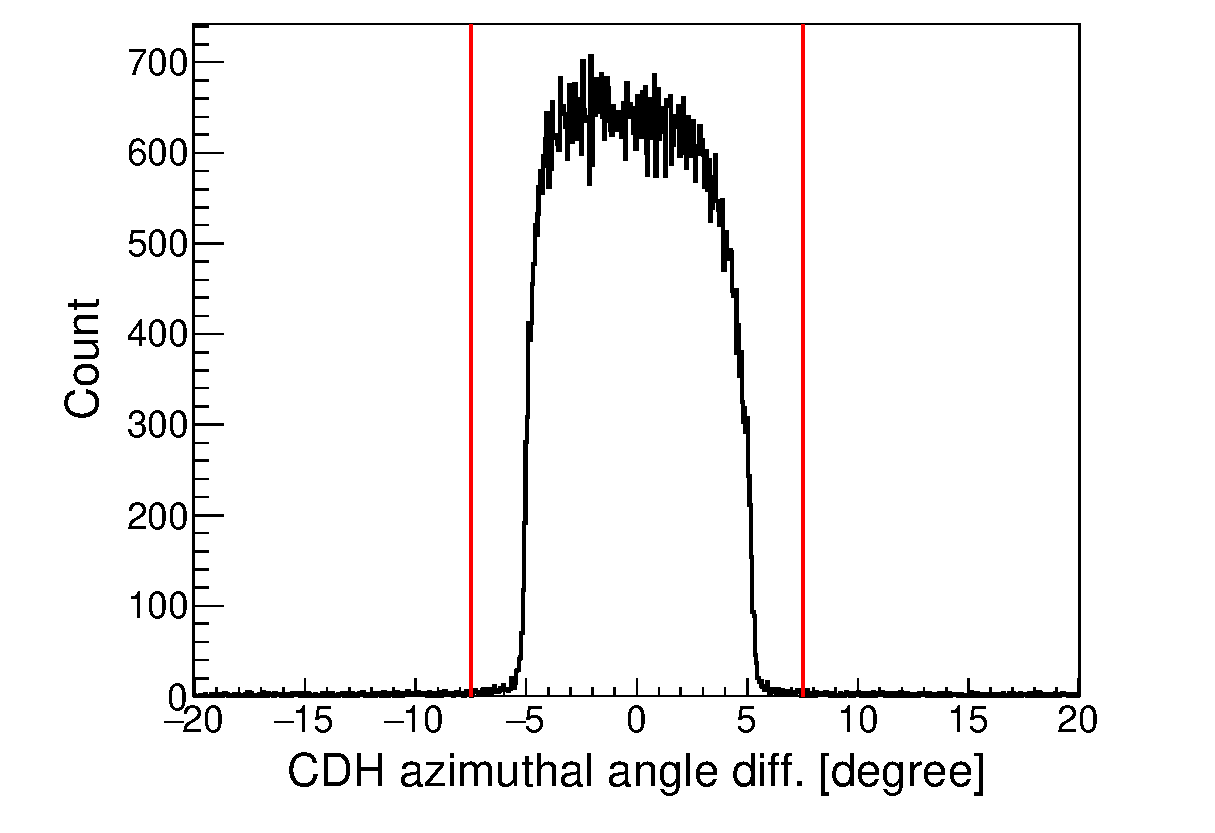
\includegraphics[width=6cm]{../pic/Dron/CDH_dphi.eps}
    \end{minipage}

    \begin{minipage}{0.5\hsize}
      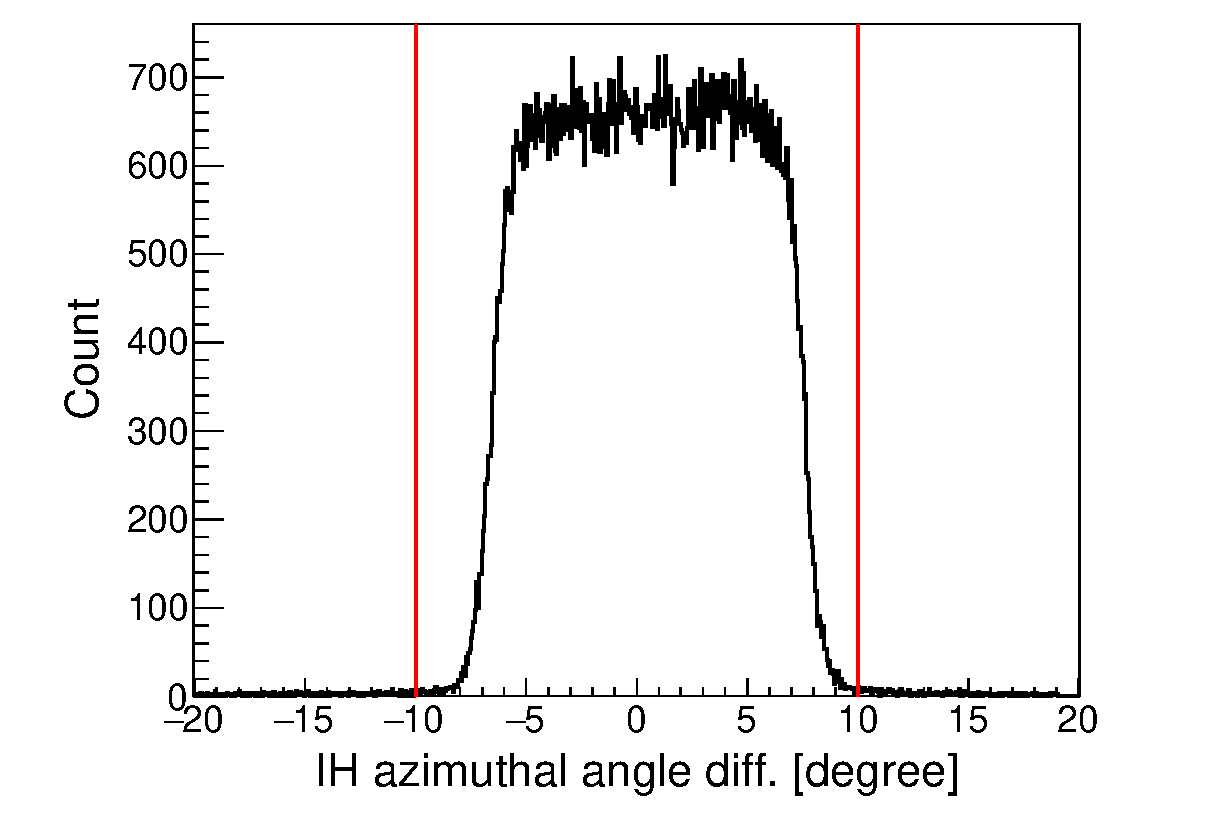
\includegraphics[width=6cm]{../pic/Dron/IH_dphi.eps}
    \end{minipage}
  \end{tabular}
  \caption{
    Left figure shows azumithal angle difference the CDH hit segment and the CDC trackin.
    Right figure shows azumithal angle difference the IH hit segment and the CDC tracking.
    The CDH and the IH segment size are $\pm5^{\circ}$ and $\pm7.5^{\circ}$, repectively.
    Acceptable region indicates red lines.
  }
  \label{fig:CDH_dphi}
\end{figure}
The CDH was installed outer side of the CDC and The IH was installed inner side of CDC.
The CDH and IH hit position can defined exported trajectory by the CDC like Fig\ref{fig:CDH_dphi}.
The CDH and the IH have 36 and 24 segments, respectively which correspond to 10 degree and 15 degree of azumithal angle.
CDC track and CDH or IH hit within $\pm7.5^{\circ}$ and $\pm10^{\circ}$  are associated, respectively.
Fig\ref{fig:CDH_dphi} shows azumithal angle matching of the CDC and the CDH and the IH.

The CDH timing infomation is used to identify of the particle.
The flight length of the T0 to the CDH is calculated in two parts, one is the T0 to the reaction vertex point which was evaluated and next is the reaction vertex point to the CDH hit position.

